\chapter{Evaluation de la capacité des méthodes développées à assimiler les données sur plusieurs applications}

\section{Objectif}

Deux adaptations du filtre EnKF ont été proposées pour être permettre l'assimilation de données pour des méthodes sans maillages. En effet, la correction à la Kalman entrainait des solutions dont le nombre de particules augmentait de manière exponentiel. Afin d'y remédier, les deux méthodes se bases  basent sur deux paradigmes : soit générer une nouvelle distribution de particule, soit approcher la solution analysée. Afin de valider ces deux approches, deux études ont été réalisées. La première présente une méthode unidimensionnelle d'un problème d'advection-diffusion. L'objectif est de mieux visialiser les différentes approches et de les comparer à une solution définies par une discrétisation eulérienne. Dans un second temps, les deux filtres sont appliqués à à un problème d'écoulement incompressible bidimensionnel non linéaire, résolu via la méthode Vortex-In-Cell (VIC) où les paramètres des filtres seront variés.

\section{Problème 1D d'advection diffusion}~\label{sec:App_1D}

Une exploration initiale est menée sur une application unidimensionnelle pour évaluer la performance des filtres. Nous définissons le problème périodique de convection-diffusion unidimensionnel sur une période de $2\pi$ suivant

\begin{equation*}
    \frac{\partial u}{\partial t}(x,t) + v \frac{\partial u}{\partial x}(x,t) = \visc \frac{\partial^2 u}{\partial x^2}(x,t),
\end{equation*}

avec $x$ la coordonnée spatiale, $v$ une vitesse constante et $\visc$ un coefficient de diffusion constant.
Pour l'application suivante, la solution de référence utilise les paramètres $v = \refv$ et $\visc = \refvisc$.
Nous définissons le noyau de chaleur périodique $2\pi$ en une dimension comme suit :

\begin{equation*}
    \phi(u, s) = \sum_{k=-\infty}^{\infty} \frac{1}{\sqrt{4 \pi s}} \exp{\left(-\frac{{(u - 2\pi k)}^2}{4s} \right)}.
\end{equation*}

Considérant une condition initiale caractérisée par une forme gaussienne exprimée comme $u^{gt}(z, 0) = \phi(z-z_0, Dt_0)$, où $\zz$, $t_0 = \frac{\sigma_0^2}{2D}$, et $\sigz$, nous dérivons la solution analytique complète en utilisant la solution de l'équation de Green :

\begin{equation*}
    u^{gt}(z, t) = \phi(z- v t - z_0, \visc (t+t_0)).
\end{equation*}

La solution analytique est succinctement décrite comme une fonction gaussienne, caractérisée par une moyenne qui se déplace à la vitesse d'advection et une déviation standard proportionnelle à $t$ et $D$. Cette solution est illustrée dans la Figure~\ref{fig:1d_analytical} à travers diverses périodes d'assimilation.

\begin{figure}[ht]
    \centering
    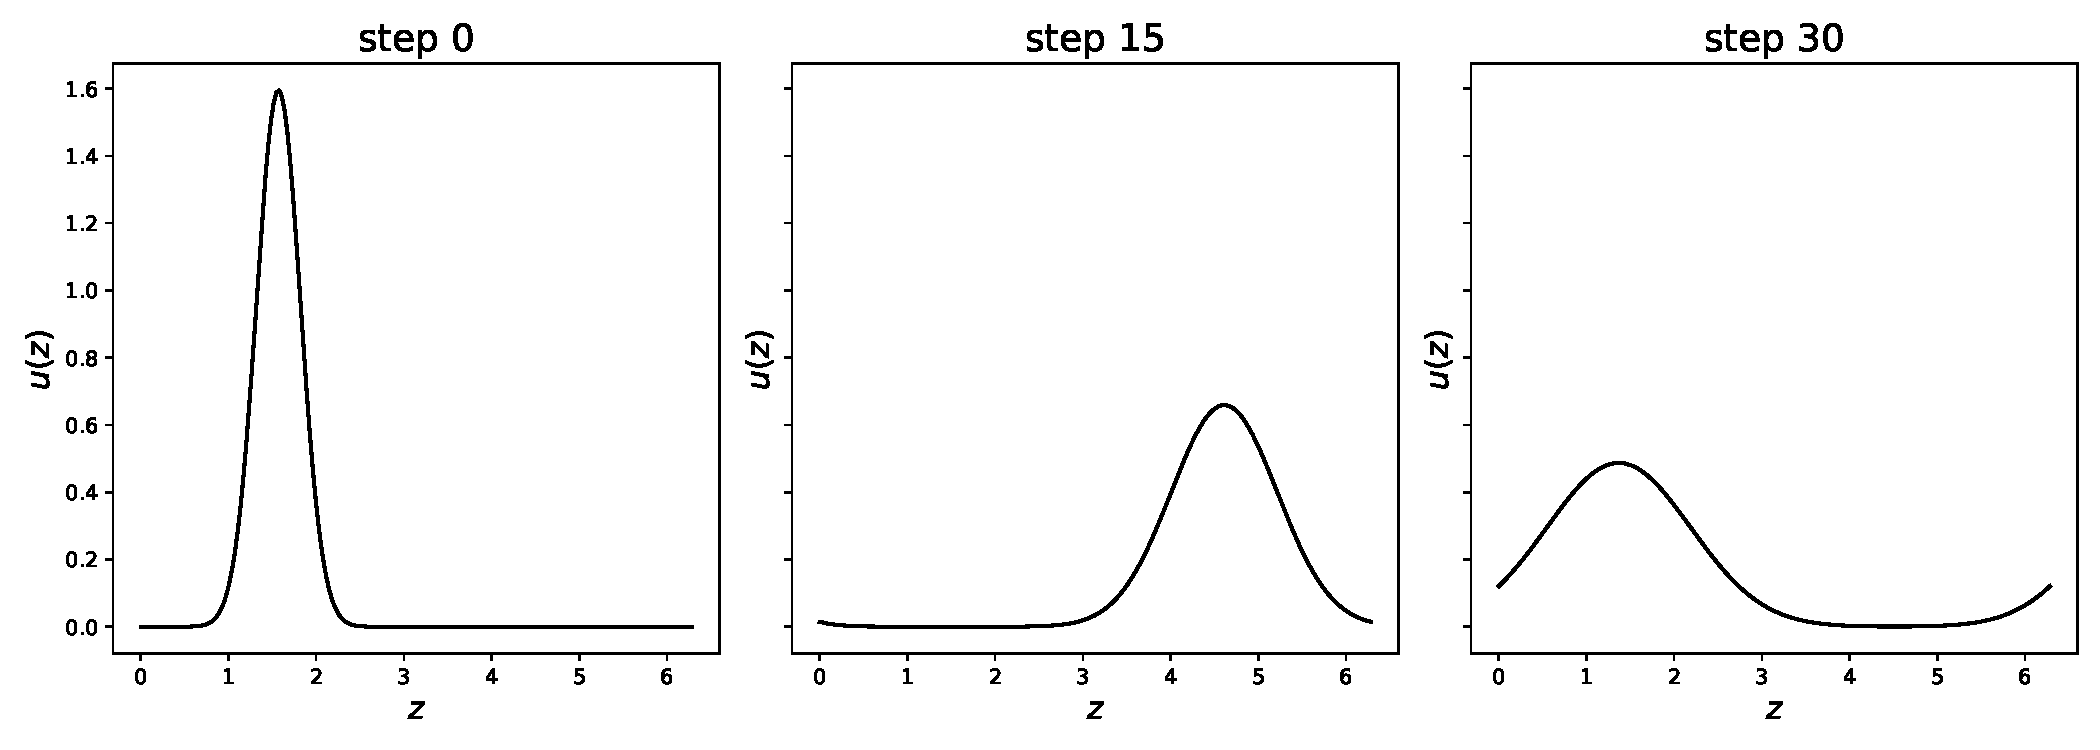
\includegraphics[width=\linewidth]{images/app1d/analytical_frame.pdf}
    \caption{La solution analytique du problème de convection-diffusion évolue au fil du temps, le dernier instantané révélant une période spatiale complète.}
    \label{fig:1d_analytical}
\end{figure}

La forme lagrangienne des équations est

\begin{equation*}
    \frac{dx_p}{dt} = v(x_p, t), \quad \frac{dU_p}{dt} = D \frac{d^2 U_p}{dx^2}
\end{equation*}

Pour résoudre le schéma de convection-diffusion, nous employons les deux étapes de l'algorithme de fractionnement visqueux. L'advection est prise en compte en mettant à jour la position de la particule avec un schéma explicite d'Euler.
D'autre part, nous utilisons une méthode de redistribution appelée la méthode d'échange de force des particules (PSE)~\cite{degond_1989,cottet_1990} pour approximer le terme laplacien $\frac{d^2 U_p}{dz^2}$.

\begin{equation*}
    D \frac{d^2 U_p}{dz^2} = D V_p \frac{d^2 u_p}{dz^2} \approx D V_p \varepsilon^{-d} \int [u(z) - u(y)] \phi_\varepsilon(y - z) dz,
\end{equation*}

Elle traite l'approximation des particules par une redistribution des intensités des particules dans leurs positions précédentes, comme suit :

\begin{equation*}
    \frac{dU_p}{dt} = D \varepsilon^{-d} V_p \sum_q (U_q - U_p) \phi_\varepsilon( z_q - z_p),
\end{equation*}

où $V_p$ est le volume de la particule $p$ et $d$ la dimension de $\Omega$.
Pour plus de détails sur le calcul, veuillez vous référer à \cite{cottet_1990}.

Pour le problème aux limites périodiques décrit dans la section \ref{App_1D}, nous définissons une fonction noyau équivalente $\phi_\varepsilon= \phi^P_g = \sum_{n=-\infty}^{+\infty} \phi_g(r - 2 \pi n )$.

Le modèle basé sur les particules utilise une discrétisation de \npart{} particules avec une taille de $h = \frac{L}{N_{\text{part}}}$ et une longueur de lissage de $\varepsilon = 1.3 h$.
Pour des raisons de comparaison, nous résolvons l'équation de convection-diffusion avec un schéma explicite de différences finies centrales discrétisé sur une grille régulière avec \ngrid{} nœuds.
\section{Bilan}